\documentclass[12pt,t,handout]{beamer}
\usepackage{graphicx}
\setbeameroption{show notes}
\setbeamertemplate{note page}[plain]
\usepackage{listings}
\usepackage{datetime}
\usepackage{url}

% specifications for presenter mode
%\beamerdefaultoverlayspecification{<+->}
%\setbeamercovered{transparent}

% math shorthand
\usepackage{bm}
\usepackage{amsmath}
\usepackage{mathtools}
\newcommand{\D}{\mathcal{D}}
\newcommand{\E}{\mathbb{E}}
\newcommand{\F}{\mathcal{F}}
\newcommand{\X}{\mathcal{X}}
\newcommand{\lik}{\mathcal{L}}
\DeclarePairedDelimiterX{\infdivx}[2]{(}{)}{%
  #1\;\delimsize\|\;#2%
}
\newcommand{\infdiv}{D\infdivx}
\DeclarePairedDelimiter{\norm}{\lVert}{\rVert}
\DeclareMathOperator*{\argmin}{arg\,min}
\DeclareMathOperator*{\argmax}{arg\,max}

% Bibliography
\usepackage{natbib}
\bibpunct{(}{)}{,}{a}{}{;}
\usepackage{bibentry}
\nobibliography*

\def\notescolors{1}
% header.tex: boring LaTeX/Beamer details + macros

% get rid of junk
\usetheme{default}
\beamertemplatenavigationsymbolsempty
\hypersetup{pdfpagemode=UseNone} % don't show bookmarks on initial view


% font
\usepackage{fontspec}
\setsansfont
  [ ExternalLocation = fonts/ ,
    UprightFont = *-regular ,
    BoldFont = *-bold ,
    ItalicFont = *-italic ,
    BoldItalicFont = *-bolditalic ]{texgyreheros}
\setbeamerfont{note page}{family*=pplx,size=\footnotesize} % Palatino for notes
% "TeX Gyre Heros can be used as a replacement for Helvetica"
% I've placed them in fonts/; alternatively you can install them
% permanently on your system as follows:
%     Download http://www.gust.org.pl/projects/e-foundry/tex-gyre/heros/qhv2.004otf.zip
%     In Unix, unzip it into ~/.fonts
%     In Mac, unzip it, double-click the .otf files, and install using "FontBook"

% named colors
\definecolor{offwhite}{RGB}{255,250,240}
\definecolor{gray}{RGB}{155,155,155}

\ifx\notescolors\undefined % slides
  \definecolor{foreground}{RGB}{255,255,255}
  \definecolor{background}{RGB}{24,24,24}
  \definecolor{title}{RGB}{107,174,214}
  \definecolor{subtitle}{RGB}{102,255,204}
  \definecolor{hilit}{RGB}{102,255,204}
  \definecolor{vhilit}{RGB}{255,111,207}
  \definecolor{lolit}{RGB}{155,155,155}
\else % notes
  \definecolor{background}{RGB}{255,255,255}
  \definecolor{foreground}{RGB}{24,24,24}
  \definecolor{title}{RGB}{27,94,134}
  \definecolor{subtitle}{RGB}{22,175,124}
  \definecolor{hilit}{RGB}{122,0,128}
  \definecolor{vhilit}{RGB}{255,0,128}
  \definecolor{lolit}{RGB}{95,95,95}
\fi
\definecolor{nhilit}{RGB}{128,0,128}  % hilit color in notes
\definecolor{nvhilit}{RGB}{255,0,128} % vhilit for notes

\newcommand{\hilit}{\color{hilit}}
\newcommand{\vhilit}{\color{vhilit}}
\newcommand{\nhilit}{\color{nhilit}}
\newcommand{\nvhilit}{\color{nvhilit}}
\newcommand{\lolit}{\color{lolit}}

% use those colors
\setbeamercolor{titlelike}{fg=title}
\setbeamercolor{subtitle}{fg=subtitle}
\setbeamercolor{institute}{fg=lolit}
\setbeamercolor{normal text}{fg=foreground,bg=background}
\setbeamercolor{item}{fg=foreground} % color of bullets
\setbeamercolor{subitem}{fg=lolit}
\setbeamercolor{itemize/enumerate subbody}{fg=lolit}
\setbeamertemplate{itemize subitem}{{\textendash}}
\setbeamerfont{itemize/enumerate subbody}{size=\footnotesize}
\setbeamerfont{itemize/enumerate subitem}{size=\footnotesize}

% page number
\setbeamertemplate{footline}{%
    \raisebox{5pt}{\makebox[\paperwidth]{\hfill\makebox[20pt]{\lolit
          \scriptsize\insertframenumber}}}\hspace*{5pt}}

% add a bit of space at the top of the notes page
\addtobeamertemplate{note page}{\setlength{\parskip}{12pt}}

% default link color
\hypersetup{colorlinks, urlcolor={hilit}}

\ifx\notescolors\undefined % slides
  % set up listing environment
  \lstset{language=bash,
          basicstyle=\ttfamily\scriptsize,
          frame=single,
          commentstyle=,
          backgroundcolor=\color{darkgray},
          showspaces=false,
          showstringspaces=false
          }
\else % notes
  \lstset{language=bash,
          basicstyle=\ttfamily\scriptsize,
          frame=single,
          commentstyle=,
          backgroundcolor=\color{offwhite},
          showspaces=false,
          showstringspaces=false
          }
\fi

% a few macros
\newcommand{\bi}{\begin{itemize}}
\newcommand{\bbi}{\vspace{24pt} \begin{itemize} \itemsep8pt}
\newcommand{\ei}{\end{itemize}}
\newcommand{\ig}{\includegraphics}
\newcommand{\subt}[1]{{\footnotesize \color{subtitle} {#1}}}
\newcommand{\ttsm}{\tt \small}
\newcommand{\ttfn}{\tt \footnotesize}
\newcommand{\figh}[2]{\centerline{\includegraphics[height=#2\textheight]{#1}}}
\newcommand{\figw}[2]{\centerline{\includegraphics[width=#2\textwidth]{#1}}}


%%%%%%%%%%%%%%%%%%%%%%%%%%%%%%%%%%%%%%%%%%%%%%%%%%%%%%%%%%%%%%%%%%%%%%
% end of header
%%%%%%%%%%%%%%%%%%%%%%%%%%%%%%%%%%%%%%%%%%%%%%%%%%%%%%%%%%%%%%%%%%%%%%

% title info
\title{Evaluating Survival Prognosis in the Presence of Immortal Time Bias}
\subtitle{\scriptsize for \textit{a meeting of the research group of
    Prof.~Sandrine Dudoit},\\ given \today}
\author{\href{https://github.com/kevinbenac}{Kevin Benac} and
        \href{https://nimahejazi.org}{Nima Hejazi}
       \\[-10pt]
       }
\institute{Group in Biostatistics \\
           University of California, Berkeley
           \\[4pt]
           %\href{https://www.stat.berkeley.edu/~nhejazi}
             %{\tt \scriptsize \color{foreground}
               %stat.berkeley.edu/\textasciitilde{}nhejazi
             %}
           %\\[4pt]
           
\includegraphics[height=20mm]{Figs/seal-berkeley.png}
           \\[-12pt]
          }
\date{
  %\href{http://nimahejazi.org}
      %{\tt \scriptsize \color{foreground} nimahejazi.org}
  %\\[-4pt]
  %\href{https://twitter.com/nshejazi}
      %{\tt \scriptsize \color{foreground} twitter/@nshejazi}
  %\\[-4pt]
  %\href{https://github.com/nhejazi}
      %{\tt \scriptsize \color{foreground} github/nhejazi}
}

%%%%%%%%%%%%%%%%%%%%%%%%%%%%%%%%%%%%%%%%%%%%%%%%%%%%%%%%%%%%%%%%%%%%%%%%%%%%%%%%

\begin{document}

% title slide
{
\setbeamertemplate{footline}{} % no page number here
\frame{
  \titlepage

  \vspace{-1em}

  \centerline{\href{https://goo.gl/Cqd9ex}{\tt \scriptsize
                                           \underline{slides}: goo.gl/Cqd9ex}}
  \vspace{-1.5em}
  \vfill \hfill 
\includegraphics[height=6mm]{Figs/cc-zero.png} \vspace*{-0.5cm}

  \note{This slide deck is meant to serve as a template for building
    presentations conveniently from a reasonable baseline.

    Slides: {\tt https://goo.gl/Cqd9ex} \\
    With notes: {\tt https://goo.gl/PFeKRH}
}
}
}

%%%%%%%%%%%%%%%%%%%%%%%%%%%%%%%%%%%%%%%%%%%%%%%%%%%%%%%%%%%%%%%%%%%%%%%%%%%%%%%%

%\begin{frame}[fragile,c]{}

%\begin{center}
%\begin{minipage}[c]{9.3cm}
%\begin{semiverbatim}
%\lstset{basicstyle=\normalsize}
%\begin{lstlisting}[linewidth=9.3cm]
  %It's always good to start with a
  %motivating example. Excerpts from
  %famous studies/papers or personal
  %communications usually do nicely.

  %It's also good practice to keep
  %things like this rather short.

  %--Nima
%\end{lstlisting}
%\end{semiverbatim}
%\end{minipage}
%\end{center}

%\note{Obviously, it's important to explain the motivating example here.}

%\end{frame}

%%%%%%%%%%%%%%%%%%%%%%%%%%%%%%%%%%%%%%%%%%%%%%%%%%%%%%%%%%%%%%%%%%%%%%%%%%%%%%%%

\begin{frame}[c]{Data and Motivation}

\begin{center}
\begin{itemize}
  \itemsep12pt
  \item Consider a data analysis scenario in which we are given survival times
    for patients recruited based on a first primary melanoma.
  \item Over the course of the observational study, an \textit{a priori} unknown
    number of the patients ($n_2$) develop a second primary melanoma prior to
    death.
  \item \textbf{Question of interest:} \textit{How does the occurrence of a
    second primary melanoma change the survival prognosis of a patient?}
\end{itemize}
\end{center}

\note{
}

\end{frame}

%%%%%%%%%%%%%%%%%%%%%%%%%%%%%%%%%%%%%%%%%%%%%%%%%%%%%%%%%%%%%%%%%%%%%%%%%%%%%%%%

\begin{frame}[c]{Preview: Summary}
\only<1>{\addtocounter{framenumber}{-1}}

\begin{center}
\begin{itemize}
  \itemsep12pt
  \item Nonparametric estimators of survival (even the NP-MLE) displays bias
    under this data-generating mechanism.
  \item The Cox proportional hazards model provides a way to mitigate this bias
    but comes with assumptions that are difficult to verify in practice.
  \item Youlden provides an approach that appears intuitive but fails to
    approach the parameter of interest.
  \item Jewell provides a correction for employing the Kaplan--Meier estimator
    in this setting.
\end{itemize}
\end{center}

\note{We'll go over this summary again at the end of the talk. Hopefully, it
  will all make more sense then.
}

\end{frame}

%%%%%%%%%%%%%%%%%%%%%%%%%%%%%%%%%%%%%%%%%%%%%%%%%%%%%%%%%%%%%%%%%%%%%%%%%%%%%%%%

\begin{frame}[c]{Survival Analysis}

\begin{center}
\begin{itemize}
  \itemsep12pt
  \item Study of the distribution of a lifetime $T$, corresponding to the time
    from a \textbf{well-defined origin} until the occurrence of a
    \textbf{well-defined event} or \textbf{endpoint}.
  \item For historical reasons, the event is often referred to as a
    \textbf{failure}.
  \item An individual for whom an event has not occurred at time $t$ is said to
    be \textbf{at risk} at time $t$.
  \item Although the term \textit{failure} is usually associated with
    \textit{death}, especially in medical research, it has to be taken in the
    broad sense of a well-defined event.
\end{itemize}
\end{center}

\note{
}

\end{frame}

%%%%%%%%%%%%%%%%%%%%%%%%%%%%%%%%%%%%%%%%%%%%%%%%%%%%%%%%%%%%%%%%%%%%%%%%%%%%%%%%

\begin{frame}[c]{Survival Analysis}

\begin{center}
\begin{itemize}
  \itemsep12pt
  \item $T$ is a non-negative random variable.
  \item If $T_1, \ldots, T_n \stackrel{iid}{\sim} T$ are observed, then we know
    that the empirical cumulative distribution function (eCDF) is the NP-MLE of
    $F_T(\cdot).$
  \item \textit{Problem:} In practice, we always have to deal with missing data
    (i.e., \textbf{censored observations}) in the context of survival data. Most
    of the time, this is merely \textbf{right-censoring}.
\end{itemize}
\end{center}

\note{
\begin{itemize}
  \item A second problem that obviously makes this estimator way too simple is
    that, like usual, covariate information should be taken into account in the
    estimation of $F_T(\cdot).$
\end{itemize}
}

\end{frame}


%%%%%%%%%%%%%%%%%%%%%%%%%%%%%%%%%%%%%%%%%%%%%%%%%%%%%%%%%%%%%%%%%%%%%%%%%%%%%%%%

\begin{frame}[c]{Survival Analysis}

\vspace{-2em}
\begin{figure}[H]
%\hspace{-3.64em}
\begin{center}
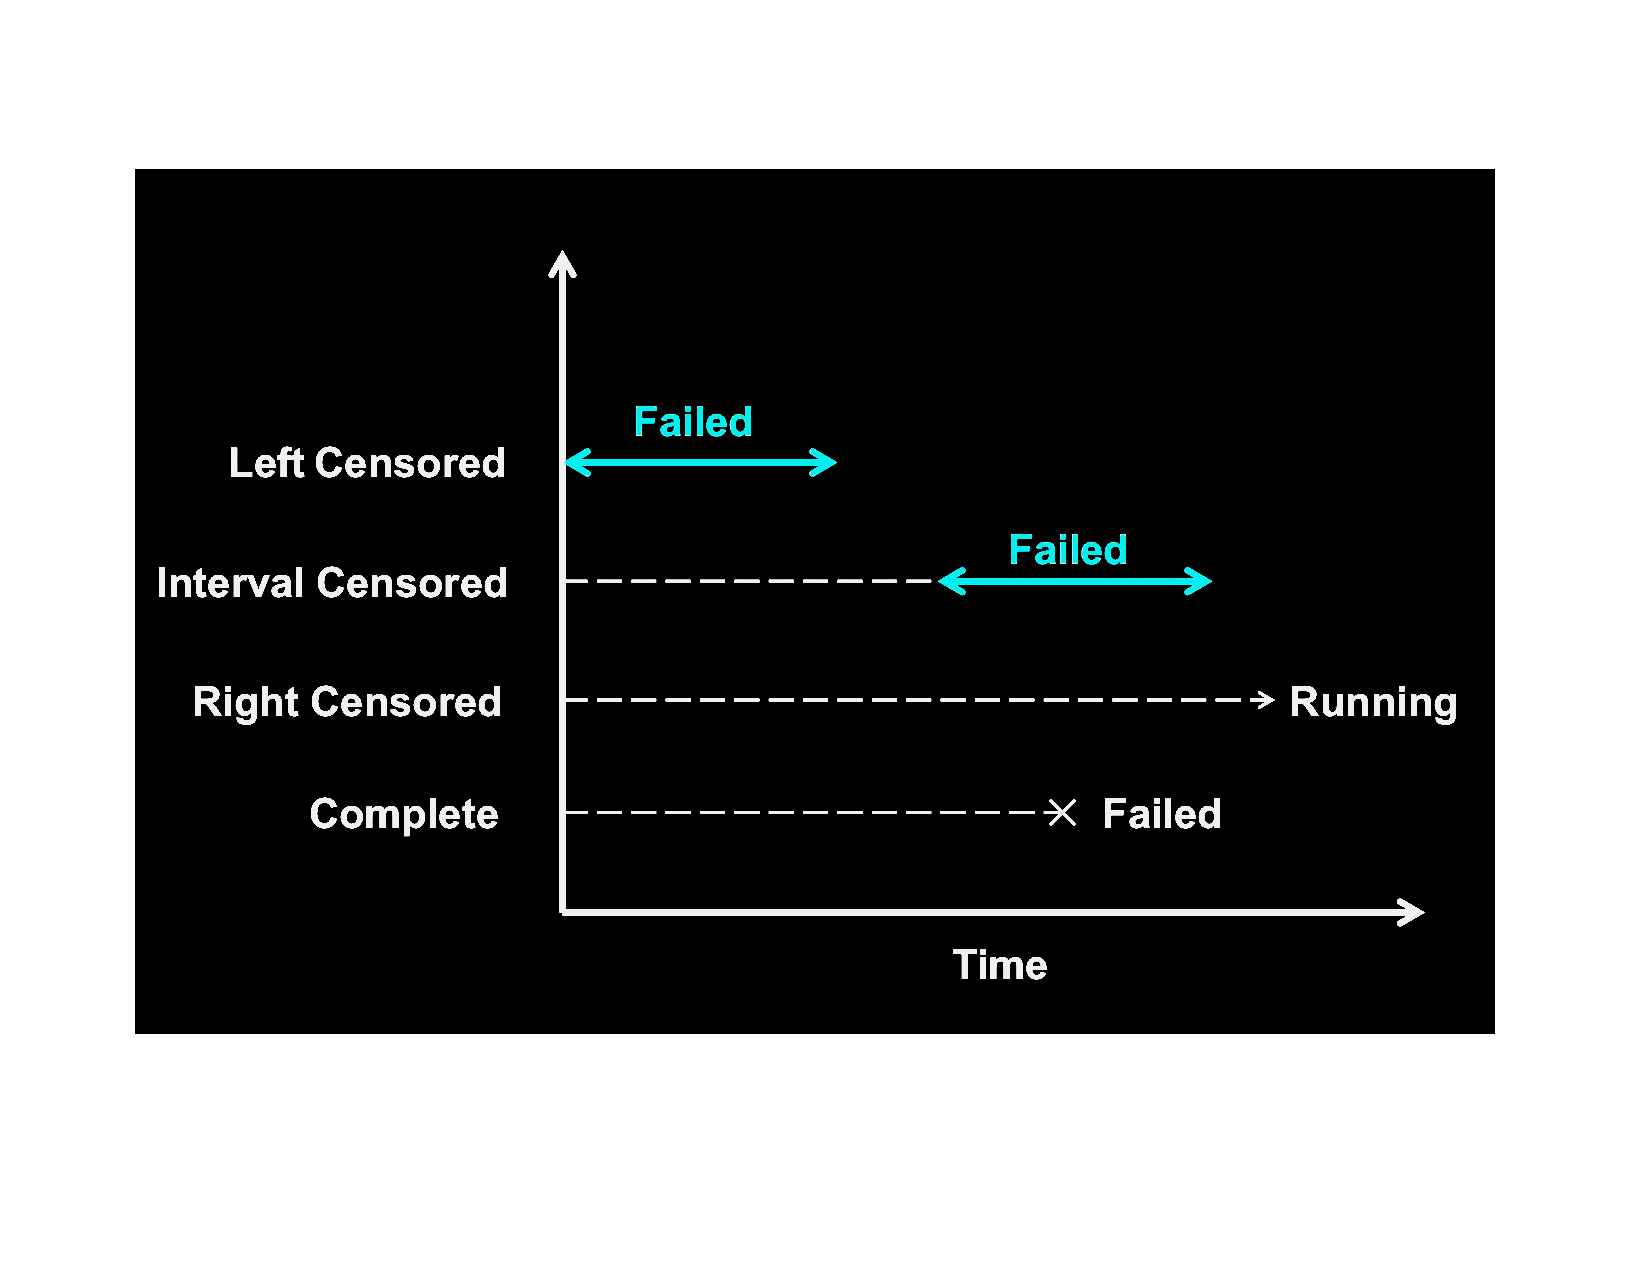
\includegraphics[width = 0.68\textwidth, angle = 270]{Figs/censoring_inv.pdf}
%\caption{\textit{Different types of censoring.} The dashed lines correspond to
  %the period during which the individual is followed; red intervals correspond
  %to time-intervals during which the individual is not followed and
  %failed.}
\end{center}
\label{fig:censoring}
\end{figure}

\note{
Caption: \textit{Different types of censoring.} The dashed lines correspond to
the period during which the individual is followed; red intervals correspond to
time-intervals during which the individual is not followed and failed.
}

\end{frame}


%%%%%%%%%%%%%%%%%%%%%%%%%%%%%%%%%%%%%%%%%%%%%%%%%%%%%%%%%%%%%%%%%%%%%%%%%%%%%%%%

\begin{frame}[c]{The Kaplan--Meier Estimator}

\begin{itemize}
  \itemsep12pt
  \item Kaplan and Meier (1958) extensively studied the case where
    right-censored data are present in survival analysis.
  \item Let us denote the distinct ordered times of observed failures by
    $$t^{(1)}<\cdots< t^{(m)},$$
\end{itemize}

\begin{center}
\begin{tabular}{ | l | c | c | c | c | }
  \hline
    Time & $t^{(1)}$  & $t^{(2)}$ & $\quad \ldots \quad$ & $t^{(m)}$ \\ \hline
    Failures & $d_1$ & $d_2$ & $\quad \ldots \quad$ & $d_{m}$ \\ \hline
    At risk & $n_1 = n$  & $n_2$ & $\quad \ldots \quad$ & $n_m$\\
  \hline
\end{tabular}
\end{center}
\note{
}

\end{frame}

%%%%%%%%%%%%%%%%%%%%%%%%%%%%%%%%%%%%%%%%%%%%%%%%%%%%%%%%%%%%%%%%%%%%%%%%%%%%%%%%


\begin{frame}[c]{The Kaplan--Meier Estimator}

If $t>0$, $t^{(i)} <t \leq t^{(i+1)}$ then we can decompose $S(t^{(i)})$ as

$$ P\left\{T> t^{(1)}\right\}P\left\{T>t^{(2)} \mid T>t^{(1)}\right\}\cdots
P\left\{ T> t^{(i)} \mid T> t^{(i-1)} \right\}.$$

The Kaplan--Meier estimator is defined as
$$
\widehat{S}(t) = \prod_{i : t(i) < t} \left(1 - \frac{d_i}{n_i}\right), \quad
t\geq 0.
$$

\note{
}

\end{frame}

%%%%%%%%%%%%%%%%%%%%%%%%%%%%%%%%%%%%%%%%%%%%%%%%%%%%%%%%%%%%%%%%%%%%%%%%%%%%%%%%

\begin{frame}[c]{The Kaplan--Meier Estimator}

\begin{center}
\begin{itemize}
  \itemsep12pt
  \item In the case of data including possible right-censoring, the Kaplan--Meier
    estimator is the NP-MLE for $S(t)$.
  \item When there is no censoring, the Kaplan--Meier estimator coincides with
    $1 - \text{eCDF}(\cdot)$.
  \item The Kaplan--Meier estimator relies on a central assumption that $T$ and
    $C$ (censoring variable) are independent, which is non-testable in practice.
\end{itemize}
\end{center}

\note{An important and problematic limitation of Kaplan--Meier is that it does
  not allow us to use covariate information.
}

\end{frame}

%%%%%%%%%%%%%%%%%%%%%%%%%%%%%%%%%%%%%%%%%%%%%%%%%%%%%%%%%%%%%%%%%%%%%%%%%%%%%%%%

\begin{frame}[c]{Hazard Function}

The \textit{hazard function} at time $t$ is defined by
$$\lambda(t) = \lim_{h \to 0}
 \frac{P\left(T< t+h \mid T\geq t \right)}{h}= \frac{f(t)}{S(t)}, \quad t > 0.$$

The hazard and the survival functions are related by
$$S(t) = \exp\left\{-\Lambda(t)\right\}, \quad t > 0,$$
where

$$\Lambda(t) = \int_0^t \lambda(s) ds, \quad t > 0$$

and is known as the \textbf{cumulative hazard function}.

\note{
}
\end{frame}

%%%%%%%%%%%%%%%%%%%%%%%%%%%%%%%%%%%%%%%%%%%%%%%%%%%%%%%%%%%%%%%%%%%%%%%%%%%%%%%%

\begin{frame}[c]{The Cox Proportional Hazards Model}

\begin{center}
\begin{itemize}
  \item The most widely used regression model in survival analysis is Cox's
    \textit{proportional hazards} model (of the hazard function):
\end{itemize}

$$
\lambda \left(t; Z = z \right) = \lambda_0(t) \exp\left(\beta^Tz \right),
\quad t\geq 0.
$$

\begin{itemize}
  \item This is a \textit{semiparametric} model: nonparametric in
    $\lambda_0(\cdot)$ but parametric in $\beta$.
\end{itemize}
\end{center}

\note{
  Note that we refer to the Cox proportional hazards model as
  \textit{semiparamtric} in the classical sense --- that is, partly
  nonparametric and partly parametric. (This is different from the sense in
  which semiparametric is used in the missing data / causal inference
  communities (e.g., J.M.~Robins, A.~Tsiatis, M.J.~van der Laan).
}

\end{frame}

%%%%%%%%%%%%%%%%%%%%%%%%%%%%%%%%%%%%%%%%%%%%%%%%%%%%%%%%%%%%%%%%%%%%%%%%%%%%%%%%

\begin{frame}[c]{Data and Motivation}

\begin{center}
\begin{itemize}
  \itemsep12pt
  \item \textit{Problem:} Efficiently estimate survival prognosis for a data
    structure exhibiting immortal time bias.
  \item \textit{Why?} Efficient estimation under a time-dependent risks bias
    presents a novel challenge that has received meager attention in the
    literature.
  \item We employ and compare
    \begin{enumerate}
      \item semiparametric estimators of survival: the Cox proportional hazards
        model (with time-varying covariates),
      \item Nonparametric estimators of survival: variations of the the
        Kaplan--Meier estimator.
    \end{enumerate}
\end{itemize}
\end{center}

\note{
We simulate data under the assumptions of the Cox proportional hazards model,
evaluating the efficiency of each estimator so as to better develop an
understanding of how to analyze the observed data we expect.
}

\end{frame}

%%%%%%%%%%%%%%%%%%%%%%%%%%%%%%%%%%%%%%%%%%%%%%%%%%%%%%%%%%%%%%%%%%%%%%%%%%%%%%%%

\begin{frame}[c]{The Cox Proportional Hazards Model}

\begin{center}
\begin{itemize}
  \itemsep12pt
  \item In the case we consider for motivation, let $U$ be the time where a
    second event occurs, then define $Z(t) = I(t > U), \quad t\geq 0.$
  \item Fitting the Cox model with $Z(t)$ as a covariate enables us to estimate
    how the risk for the patient changes after the appearance of the second
    melanoma.
\end{itemize}
\end{center}

\note{
  The Cox model may be extended to deal with time-dependent covariates,
  Martingale theory, etc.
}

\end{frame}

%%%%%%%%%%%%%%%%%%%%%%%%%%%%%%%%%%%%%%%%%%%%%%%%%%%%%%%%%%%%%%%%%%%%%%%%%%%%%%%%

\begin{frame}[c]{Methodology --- Cox Regression}

\begin{center}
\begin{itemize}
  \itemsep12pt
  \item We simulate observed data under the assumptions of the Cox model a total
    of $10,000$ times, averaging the estimated survival across all observed time
    points for each fit of the Cox proportional hazards regression.
  \item Recall that Cox regression estimates the hazard at a given time,
    assuming a simplistic relationship between hazards for events of interest.
  \item This borrows information across the two groups to estimate survival ---
    that is, groups experiencing a single primary melanoma and those with two
    both inform estimation of survival.
  \item We account for transitions between the two groups by way of a
    \textit{time-varying covariate}.
\end{itemize}
\end{center}

\note{
}

\end{frame}

%%%%%%%%%%%%%%%%%%%%%%%%%%%%%%%%%%%%%%%%%%%%%%%%%%%%%%%%%%%%%%%%%%%%%%%%%%%%%%%%

\begin{frame}[c]{Results --- Cox Proportional Hazards}

\begin{center}
\begin{figure}[H]
\begin{center}
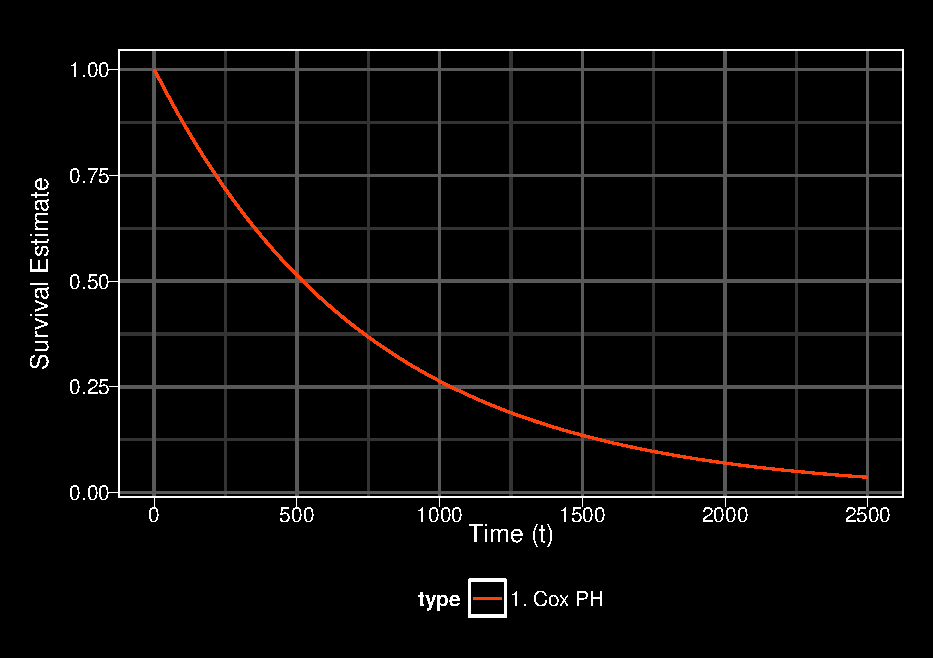
\includegraphics[width=\textwidth]{Figs/s1_cox.pdf}
\end{center}
%\caption{\textit{Performance of the Cox regression estimator}}\label{s1_cox}
\end{figure}
\end{center}

\note{
}

\end{frame}

%%%%%%%%%%%%%%%%%%%%%%%%%%%%%%%%%%%%%%%%%%%%%%%%%%%%%%%%%%%%%%%%%%%%%%%%%%%%%%%%

\begin{frame}[c]{Methdology --- Kaplan--Meier (Youlden)}

\begin{center}
\begin{itemize}
  \itemsep12pt
  \item In pratice it's impossible to know if assumptions of the Cox model hold
    for a given data-generating process we encounter ``in the wild.''
  \item This makes the use of a nonparametric approach highly desirable, so,
    \textit{how might we formulate a Kaplan--Meier estimator for this setting}?
  \item Recall that we cannot provide covariate information when fitting
    Kaplan--Meier estimators, let alone time-varying disease status.
  \item \textit{Proposal:} Fit a Kaplan--Meier estimator for patients that
    experience only a single primary melanoma.
\end{itemize}
\end{center}

\note{
We expect that this will recover the survival function for the risk conferred by
experiencing a single primary melanoma.
}

\end{frame}

%%%%%%%%%%%%%%%%%%%%%%%%%%%%%%%%%%%%%%%%%%%%%%%%%%%%%%%%%%%%%%%%%%%%%%%%%%%%%%%%

\begin{frame}[c]{Results --- Kaplan--Meier (Youlden)}

\begin{center}
\begin{figure}[H]
\begin{center}
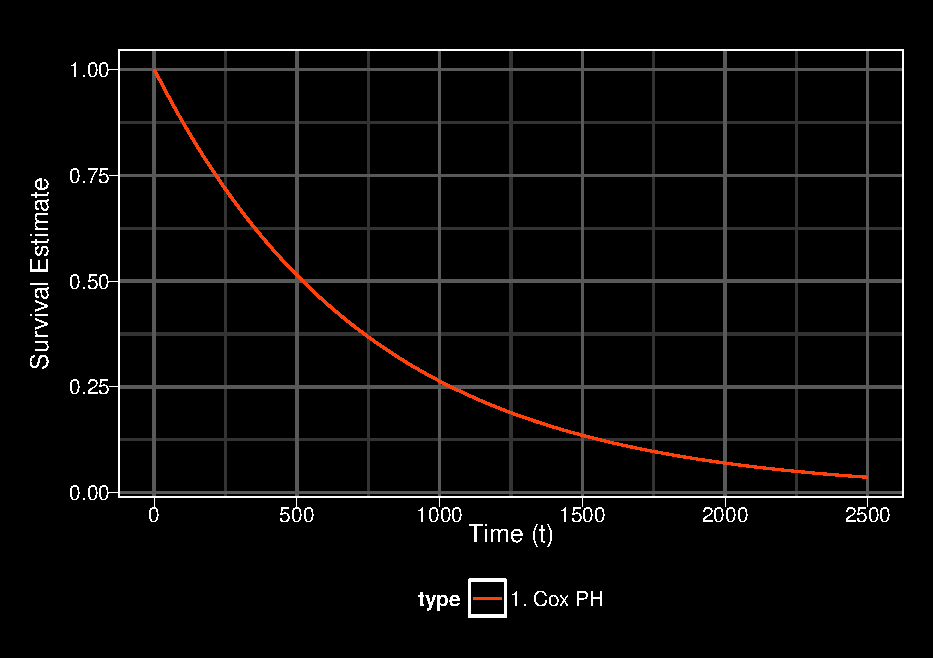
\includegraphics[width=\textwidth]{Figs/s1_cox.pdf}
\end{center}
%\caption{\textit{Performance of the Cox regression estimator}}\label{s1_cox}
\end{figure}
\end{center}

\note{
}

\end{frame}

%%%%%%%%%%%%%%%%%%%%%%%%%%%%%%%%%%%%%%%%%%%%%%%%%%%%%%%%%%%%%%%%%%%%%%%%%%%%%%%%

\begin{frame}[c]{Results --- Kaplan--Meier (Youlden)}

\begin{center}
\begin{figure}[H]
\begin{center}
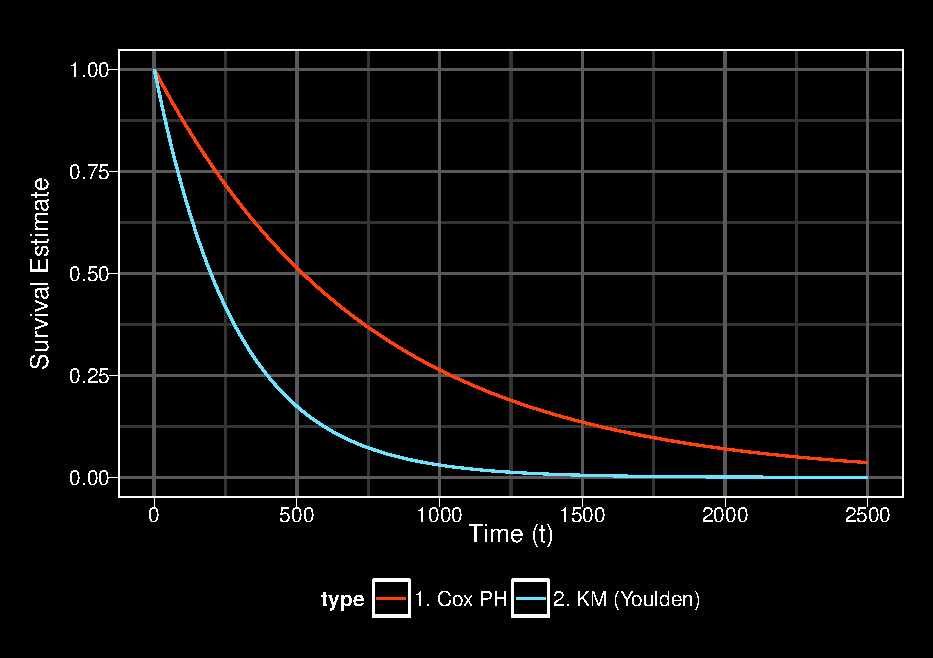
\includegraphics[width=\textwidth]{Figs/s1_cox_youlden.pdf}
\end{center}
%\caption{\textit{Comparison of the Cox PH regression estimator and Youlden's
    %proposed Kaplan--Meier estimator}}\label{s1_cox_youlden}
\end{figure}
\end{center}

\note{
}

\end{frame}

%%%%%%%%%%%%%%%%%%%%%%%%%%%%%%%%%%%%%%%%%%%%%%%%%%%%%%%%%%%%%%%%%%%%%%%%%%%%%%%%

\begin{frame}[c]{Methdology --- Kaplan--Meier (Jewell)}

\begin{center}
\begin{itemize}
  \itemsep12pt
  \item The difference between the Kaplan--Meier and Cox regression estimates of
    survival is quite striking.
  \item Given that the assumptions of the Cox model hold, we can evaluate
    Kaplan--Meier relative to Cox --- why is KM so strongly biased?
  \item Recall that we \textit{chose} to discard the second group when fitting
    our chosen KM estimator.
  \item Including such observations when fitting our KM estimator should
    \textit{de-bias} the early (in time) estimates.
\end{itemize}
\end{center}

\note{
\begin{itemize}
  \item It appears that the Youlden approach displays a great degree of bias
    across all observed times.
  \item We need a better way in which to estimate survival --- one that accounts
    for the time-varying group status.
  \item Importantly, all patients in the second group are guaranteed to survive
    until their occurrence of the second primary melanoma.
\end{itemize}
}

\end{frame}

%%%%%%%%%%%%%%%%%%%%%%%%%%%%%%%%%%%%%%%%%%%%%%%%%%%%%%%%%%%%%%%%%%%%%%%%%%%%%%%%

\begin{frame}[c]{Results --- Kaplan--Meier (Jewell)}

\begin{center}
\begin{figure}[H]
\begin{center}
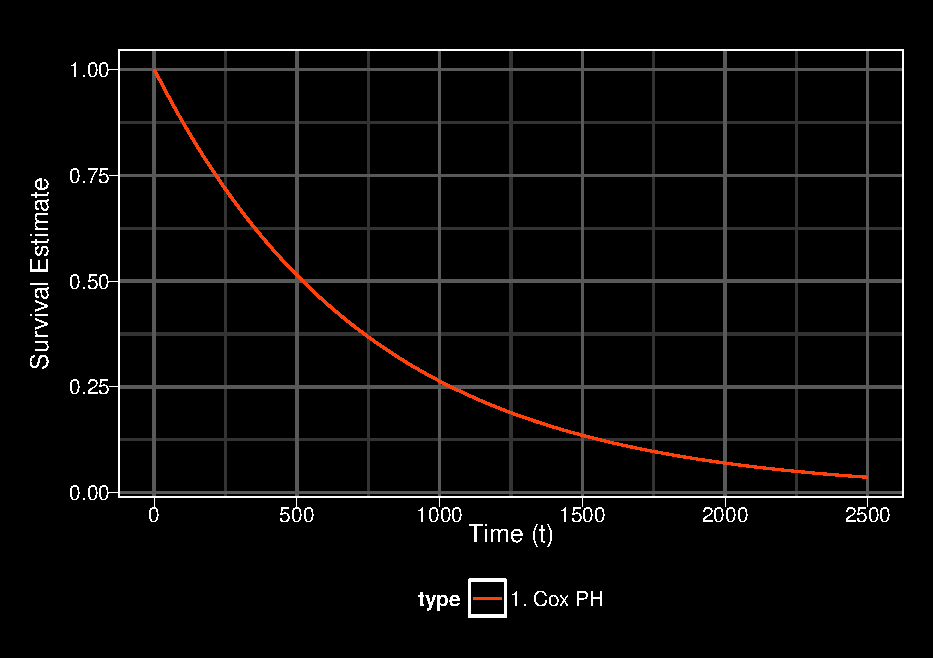
\includegraphics[width=\textwidth]{Figs/s1_cox.pdf}
\end{center}
%\caption{\textit{Performance of the Cox regression estimator}}
\label{fig:s1_cox}
\end{figure}
\end{center}

\note{
}

\end{frame}

%%%%%%%%%%%%%%%%%%%%%%%%%%%%%%%%%%%%%%%%%%%%%%%%%%%%%%%%%%%%%%%%%%%%%%%%%%%%%%%%

\begin{frame}[c]{Results --- Kaplan--Meier (Jewell)}

\begin{center}
\begin{figure}[H]
\begin{center}
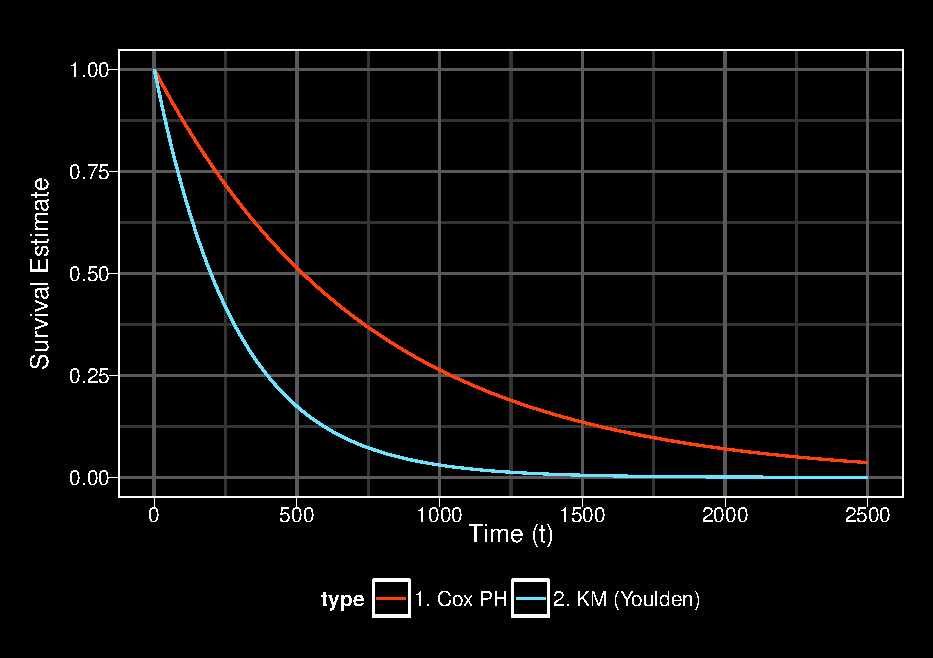
\includegraphics[width=\textwidth]{Figs/s1_cox_youlden.pdf}
\end{center}
%\caption{\textit{Comparison of the Cox PH regression estimator and Youlden's
    %proposed Kaplan--Meier estimator}}
\label{fig:s1_cox_youlden}
\end{figure}
\end{center}

\note{
}

\end{frame}

%%%%%%%%%%%%%%%%%%%%%%%%%%%%%%%%%%%%%%%%%%%%%%%%%%%%%%%%%%%%%%%%%%%%%%%%%%%%%%%%

\begin{frame}[c]{Results --- Kaplan--Meier (Jewell)}

\begin{center}
\begin{figure}[H]
\begin{center}
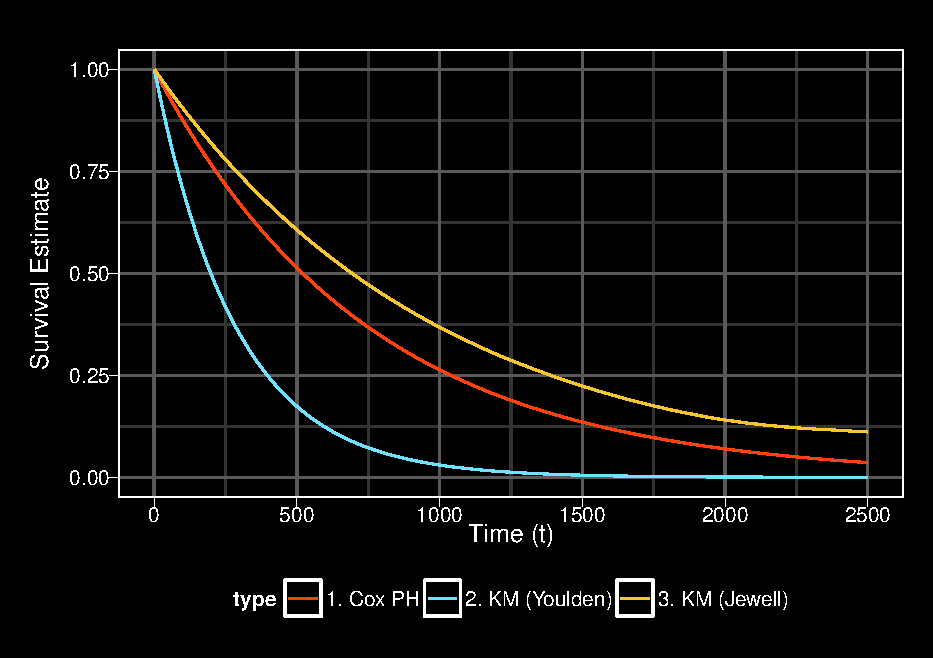
\includegraphics[width=\textwidth]{Figs/s1_cox_youlden_jewell.pdf}
\end{center}
%\caption{\textit{Comparison of the Cox PH, Youlden's Kaplan--Meier, and Jewell's
    %Kaplan--Meier estimators}}
\label{fig:s1_cox_youlden_jewll}
\end{figure}
\end{center}

\note{
}

\end{frame}

%%%%%%%%%%%%%%%%%%%%%%%%%%%%%%%%%%%%%%%%%%%%%%%%%%%%%%%%%%%%%%%%%%%%%%%%%%%%%%%%

\begin{frame}[c]{Discussion}

\begin{center}
\begin{itemize}
  \itemsep12pt
  \item Each of three estimators provides strikingly different estimates of
    survival across the observed times.
  \item Since the assumptions of the Cox model hold in our simulation, we can
    evaluate results from each of the nonparametric KM estimators relative to
    those from Cox PH.
  \item Further/ongoing investigation: \textit{How does the relative performance
    of these estimators differ when the assumptions of the Cox model do not
    hold?}
\end{itemize}
\end{center}

\note{
}

\end{frame}

%%%%%%%%%%%%%%%%%%%%%%%%%%%%%%%%%%%%%%%%%%%%%%%%%%%%%%%%%%%%%%%%%%%%%%%%%%%%%%%%

\begin{frame}[c]{Discussion}

\begin{center}
\begin{itemize}
  \itemsep12pt
  \item Our initial KM proposal exhibited strong bias, underestimating survival
    at all observed times, with a particularly noticeable bias early on.
  \item The corrected KM estimator, which draws on information from both groups,
    provides better estimates early in time, but displays a stronger positive
    bias at later times (overestimating survival).
\end{itemize}
\end{center}

\note{
}

\end{frame}

%%%%%%%%%%%%%%%%%%%%%%%%%%%%%%%%%%%%%%%%%%%%%%%%%%%%%%%%%%%%%%%%%%%%%%%%%%%%%%%%

\begin{frame}[c]{Review: Summary}

\begin{center}
\begin{itemize}
  \itemsep12pt
  \item Nonparametric estimators of survival (even the NP-MLE) displays bias
    under this data-generating mechanism.
  \item The Cox proportional hazards model provides a way to mitigate this bias
    but comes with assumptions that are difficult to verify in practice.
  \item Youlden provides an approach that appears intuitive but fails to
    approach the parameter of interest.
  \item Jewell provides a correction for employing the Kaplan--Meier estimator
    in this setting.
\end{itemize}
\end{center}

\note{It's always good to include a summary.}

\end{frame}

%%%%%%%%%%%%%%%%%%%%%%%%%%%%%%%%%%%%%%%%%%%%%%%%%%%%%%%%%%%%%%%%%%%%%%%%%%%%%%%%

% don't want dimming with references
\setbeamercovered{}
\beamerdefaultoverlayspecification{}

\begin{frame}[c,allowframebreaks]{References}

\bibliographystyle{apalike}
\nocite{*}
\bibliography{references}

%\note{Here's some work we've talked about. Go check these out if interested.}

\end{frame}

%%%%%%%%%%%%%%%%%%%%%%%%%%%%%%%%%%%%%%%%%%%%%%%%%%%%%%%%%%%%%%%%%%%%%%%%%%%%%%%%

\begin{frame}{Acknowledgments}

\vspace{18pt}

\begin{tabular}{@{}l@{\hspace{1.5cm}}l@{}}
Nicholas P.~Jewell & \footnotesize \lolit University of California, Berkeley\\
%Collaborator, the second \\
%Collaborator, the third \\

\\[2ex]

%Collaborator, the first & \footnotesize \lolit University or Institution 2 \\
%Collaborator, the second \\
\end{tabular}

%\vspace{10mm}

%Funding source?

\note{
}

\end{frame}

%%%%%%%%%%%%%%%%%%%%%%%%%%%%%%%%%%%%%%%%%%%%%%%%%%%%%%%%%%%%%%%%%%%%%%%%%%%%%%%%

\begin{frame}[c]{Thank you. Questions?}

\begin{center}
\begin{itemize}
  \itemsep12pt
  \item Nonparametric estimators of survival (even the NP-MLE) displays bias
    under this data-generating mechanism.
  \item The Cox proportional hazards model provides a way to mitigate this bias
    but comes with assumptions that are difficult to verify in practice.
  \item Youlden provides an approach that appears intuitive but fails to
    approach the parameter of interest.
  \item Jewell provides a correction for employing the Kaplan--Meier estimator
    in this setting.
\end{itemize}
\end{center}

\note{It's good to include a summary when taking questions.}

\end{frame}

%%%%%%%%%%%%%%%%%%%%%%%%%%%%%%%%%%%%%%%%%%%%%%%%%%%%%%%%%%%%%%%%%%%%%%%%%%%%%%%%

\end{document}

